\documentclass[french]{article}

% Encodage et langue
\usepackage[utf8]{inputenc}
\usepackage[T1]{fontenc}
\usepackage[french]{babel}

% Mise en page
\usepackage{geometry}
\geometry{margin=2.5cm}

% Styles
\usepackage{fancyhdr}
\usepackage{graphicx}
\usepackage{helvet}
\usepackage{hyperref}
\usepackage{listings}
\usepackage{titlesec}
\usepackage{xcolor}

\renewcommand{\familydefault}{\sfdefault}
\newcommand{\newLine}{\vspace{0.2cm}}


% Style du code C#
\definecolor{codegray}{rgb}{0.5,0.5,0.5}
\definecolor{backcolour}{rgb}{0.95,0.95,0.92}
\lstdefinelanguage{CSharp}{
  morekeywords={abstract,event,new,struct,as,explicit,null,switch,
  base,extern,object,this,bool,false,operator,throw,
  break,finally,out,true,byte,fixed,override,try,
  case,float,params,typeof,catch,for,private,uint,
  char,foreach,protected,ulong,checked,goto,public,unchecked,
  class,if,readonly,unsafe,const,implicit,ref,ushort,
  continue,in,return,using,decimal,int,sbyte,virtual,
  default,interface,sealed,volatile,delegate,internal,short,void,
  do,is,sizeof,while,double,lock,stackalloc,
  else,long,static,enum,namespace,string},
  sensitive=true,
  morecomment=[l]{//},
  morecomment=[s]{/*}{*/},
  morestring=[b]",
}
\lstset{
  language=CSharp,
  backgroundcolor=\color{backcolour},
  basicstyle=\ttfamily\footnotesize,
  keywordstyle=\color{blue}\bfseries,
  commentstyle=\color{codegray}\itshape,
  stringstyle=\color{red},
  breaklines=true,
  numbers=left,
  numberstyle=\tiny\color{gray},
  frame=single,
  tabsize=2
}

% En-tête et pied de page
\pagestyle{fancy}
\fancyhf{}
\fancyhead[L]{Documentation Technique}
\fancyhead[R]{Projet C\#}
\fancyfoot[C]{\thepage}

\begin{document}

% Page de garde moderne
\begin{titlepage}
    \centering
    % Ligne colorée décorative
    \vspace*{2cm}
    {\color{blue}\rule{\textwidth}{1.5pt}}\par
    \vspace{1cm}
    
    % Titre principal
    {\Huge\bfseries Documentation Technique\par}
    \vspace{0.5cm}
    {\Large Projet C\# – Jeu *Doodle Jump*\par}
    
    \vspace{1cm}
    {\color{blue}\rule{0.6\textwidth}{1pt}}\par
    \vspace{2cm}
    
    % Infos auteur
    {\Large \textbf{Auteur :} Etienne Caulier \par}
    \vspace{0.5cm}
    {\Large \textbf{Date :} \today \par}
    
    \vfill
    
    % Logo ou image optionnelle
    % \includegraphics[width=0.35\textwidth]{logo.png}\par
    
    \vspace{1cm}
    {\large CFPT Informatique \par}
    
    \vspace*{2cm}
\end{titlepage}


% Sommaire
\tableofcontents
\newpage

\section{\textit{Doodle Jump} en C\#}
Le projet consiste à développer une version du jeu \textbf{Doodle Jump} en C\#, en utilisant une approche orientée objet et un moteur graphique 2D. \newline

Le joueur contrôle un personnage qui saute automatiquement et dont l’objectif est de monter le plus haut possible en utilisant des plateformes.

\subsection{Objectifs du projet}
\begin{itemize}
	\item Mettre en pratique la programmation orientée objet en C\#.
	\item Gérer la \textbf{physique de base} (gravité, collisions, déplacements).
	\item Implémenter une \textbf{boucle de jeu fluide} (mises à jour et rendu en temps réel).
	\item Développer une \textbf{interface simple et intuitive} avec un score affiché à l’écran.
	\item Offrir une \textbf{expérience de jeu amusante et progressive} inspirée de l’original Doodle Jump.
	\item \textbf{Sauvegarde} de la partie en locale avec du \textit{JSON}.
\end{itemize}

\section{Technologies utilisées}
\begin{itemize}
	\item \textbf{Framework :} MonoGame.
	\item \textbf{Langage de programmation :} C\#.
	\item \textbf{Environnement de développement :} Visual Studio.
	\item \textbf{Outils de versionnalisation :} GitHub.
\end{itemize}

\section{Analyse et conception}
\subsection{Description des fonctionnalités}
Le jeu repose sur plusieurs mécanismes clés :
\begin{itemize}
	\item \textbf{Gravité et sauts :} le personnage subit une gravité constante et rebondit lorsqu’il touche une plateforme.
	\item \textbf{Sprites 2D :} les éléments visuels (personnage, plateformes, arrière-plan, bonus, ennemis) sont représentés par des sprites 2D.
	\item \textbf{Défilement vertical infini :} le décor se génère de manière continue pour donner une impression de progression infinie vers le haut.
	\item \textbf{Interactions :}
	      \begin{itemize}
		      \item plateformes fixes ou mobiles,
		      \item bonus (ressorts, jetpacks, etc.) \textbf{si j'ai le temps !},
		      \item obstacles et ennemis à éviter ou éliminer.
	      \end{itemize}
	\item \textbf{Score :} le joueur accumule des points en fonction de la hauteur atteinte.
\end{itemize}

\subsection{Diagramme UML}
Le diagramme UML suivant représente la structure des principales classes du jeu :
\begin{itemize}
	\item \textbf{Player :} Gère les actions du joueur.
	\item \textbf{Enemy :} Gère les comportements des ennemis.
	\item \textbf{Projectile :} Représente les tirs des personnages.
	\item \textbf{GameState :} Gère les états du jeu (menu, jeu en cours, fin de partie)
\end{itemize}


\begin{center}
    \vspace{1cm} % marge au-dessus
    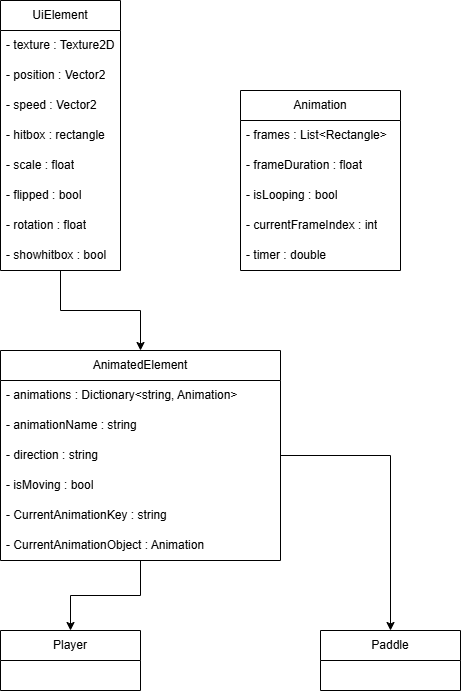
\includegraphics[width=10cm]{../Diagrammes/classes.png}
    \vspace{1cm} % marge en dessous
\end{center}






% \section{Exemple de code}
% Voici un exemple en C\# :

% \begin{lstlisting}
% // Exemple simple en C#
% public class Compte {
%     public string Nom { get; set; }
%     public decimal Solde { get; set; }

%     public void Retirer(decimal montant) {
%         if (montant <= Solde) {
%             Solde -= montant;
%         }
%     }
% }
% \end{lstlisting}

\end{document}